\SetPicSubDir{ch-methodology}
\SetExpSubDir{ch-methodology}

\chapter{Methodology}
\label{methodology}

\section{Solvers}
We will employ five QUBO-solving-methods:
\begin{enumerate}
    \item Quantum Annealing
    \item Neural Network Quantum States
    \item Quantum Approximate Optimization Algorithm
    \item GUROBI Optimizer
    \item Fixstars Amplify QUBO Solver
\end{enumerate}
The following sections will provide more information on the solvers used for each method.

\subsection{Quantum Annealing}
We will use quantum annealers from D-wave Systems as the solver for Quantum Annealing. D-Wave Systems, a Canadian-based company, currently produces the most popular commercially available quantum annealing hardware and uses superconducting qubits to represent binary variables in their annealers \cite{b14}.  Given a target QUBO problem to solve, the process for using a D-Wave Systems Quantum Processing Unit (QPU) is as follows:

\begin{enumerate}
    \item \textbf{Problem Definition} QUBO problem is first converted to its corresponding Ising model Hamiltonian on the local device.
    \item \textbf{Minor Embedding} As the Quantum Processing Unit (QPU) used by D-Wave is not fully connected as shown in \autoref{pegasustopology}, a single variable in the Ising model may need to be represented by multiple qubits called a \textit{chain} which are forced to return the same value with large interaction terms \cite{b16}. This will be done with an embedder provided by the D-wave library.
    \item \textbf{Programming} The parameters of the annealing process are set, which consists of the bias for each qubit (represents magnetic field acting on each qubit) and coupler strength (represents variable interaction).
    \item \textbf{Initialization} The QPU is initialized in the ground state of an easy-to-implement initial Hamiltonian. The qubits are prepared to be in a superposition of all possible states.
    \item \textbf{Annealing} The system evolves with a time-varying Hamiltonian.
    \item \textbf{Readout of solution} The spin values of the qubits are measured and stored as a possible solution.
    \item \textbf{Resample} As the finite-time quantum annealing process does not guarantee that the system ends up in the ground state, we repeat the sampling to obtain many possible solutions that are likely to be the ground state of the initial Hamiltonian.
\end{enumerate}
\begin{figure}[h!]
    \centering
    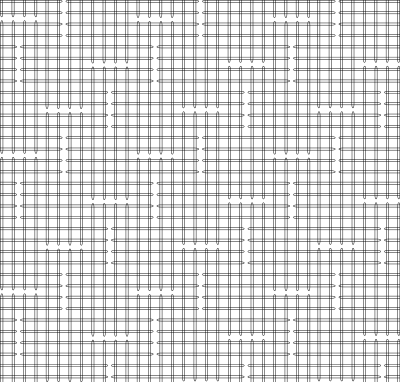
\includegraphics[width=0.5\linewidth]{images/pegasus_topology.png}
    \caption[A view of the D-Wave pegasus topology---each line represents a qubit and intersections represent available couplers]{A view of the D-Wave pegasus topology where each line represents a qubit and intersections represent available couplers~\protect\cite{dwaveadvantage}}
    \label{pegasustopology}
\end{figure}
The experiments will be conducted with the D-Wave Advantage 4.1 QPU with up to 5640 qubits and 40484 couplers \cite{dwaveadvantage}. The QPU operates at a temperature of approximately $12$mK and is built with "a network of tunably coupled rf superconducting quantum–interference device (rf-SQUID) qubits" arranged with the Pegasus graph topology that allows for up to 15 couplers per qubit, shown in \autoref{pegasustopology}. The system Hamiltonian as a function of $s$, the normalized anneal fraction, is:
\begin{equation}
    \label{eqn:dwavehamiltonian}
    H(s) = -\frac{A(s)}{2}\left(\sum_{i} \Hat{\sigma}_x^{(i)}\right) + \frac{B(s)}{2}\left(\sum_{i}h_i \Hat{\sigma}_z^{(i)}\ + \sum_{i > j}J_{i,j} \Hat{\sigma}_z^{(i)}\Hat{\sigma}_z^{j)}\right)
\end{equation}
where functions $A(s)$ and $B(s)$ used in the Advantage 4.1 QPU are shown in \autoref{dwaveannealing} with $A(s) >> B(s)$ when $s=0$ and $B(s) >> A(s)$ when $s=1$ and have an energy scale of around $10^{-24} J$.
\begin{figure}[h!]
    \centering
    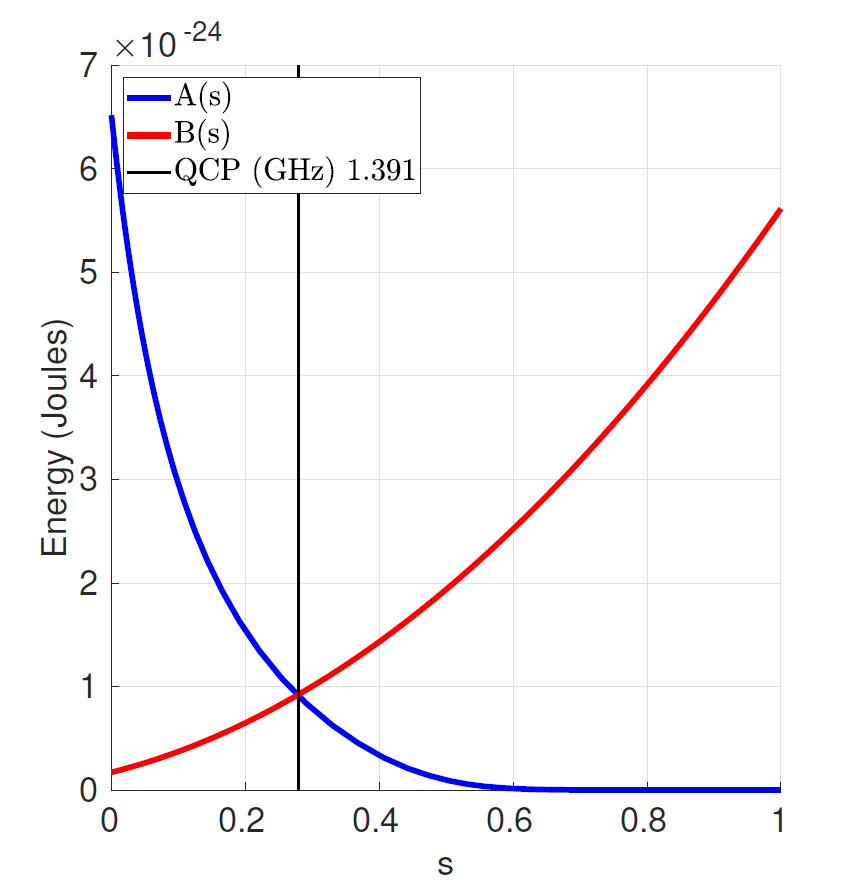
\includegraphics[width=0.6\linewidth]{images/dwave_annealing.png}
    \caption[Annealing functions $A(s)$ and $B(s)$ as a function of the normalized anneal fraction $s$]{Annealing functions $A(s)$ and $B(s)$ as a function of the normalized anneal fraction $s$~\protect\cite{dwaveadvantage}}
    \label{dwaveannealing}
\end{figure}
We will use the default annealing time of $20\mu s$ with $1000$ repeated samplings (number of reads). The candidate solution will be taken as the best solution among the $1000$ sampled configurations.


\subsection{Neural-Network Quantum States}
We will adopt the Python library MAPALUS for implementing the Neural-Network Quantum States \cite{b25}. MAPALUS uses the Tensorflow library and enables parallel execution on general-purpose graphics processing units (GPUs) for quicker sampling. In this section, we will use the Restricted Boltzmann Machine (with $5n$ hidden nodes and the sigmoid activation function) as the underlying architecture for the NNQS. 

To solve a given input QUBO problem, the NNQS will be used to simulate a quantum annealing process with a time-dependent Hamiltonian that follows \autoref{eqn:annealinghamiltonian}. Since the equations for $A(s)$ and $B(s)$ are not available, we employ a curve-fitting process to obtain analytical functions for use in the NNQS. The fitted functions used are $A(s) = 1.11e^{-7.06s} + -0.00569$ and $B(s)= 0.680s^2 + 0.288s + 0.0305$, details on the curve fitting process are available in \autoref{appendix:curvefitting}.

\begin{algorithm}
    \begin{algorithmic}
    \Require Problem Hamiltonian $\hat{H}_c$
    \Ensure Trained NNQS
    \State Initialize NNQS with random weights;
    \For {$s \in [0.1, 1.0]$ step $0.1$}
    \State Set $H(s) \leftarrow A(s)\hat{H}_0 + B(s)\hat{H}_c$;
    \State Train NNQS on $H(s)$ until convergence or until epoch limit of $100$ is reached;
    \EndFor
    \end{algorithmic}
    \caption{NNQS Progressive Training}
    \label{alg:progressive}
\end{algorithm}

The NNQS will be trained with a progressive training schedule that mimics the quantum annealing process and follows \autoref{alg:progressive}. $\hat{H}_c$ is the problem Hamiltonian and $\hat{H}_0$ is a Hamiltonian with linear biases as $1$ and no quadratic terms. The normalized anneal fraction $s$ is increased in small steps while the NNQS is trained until convergence or until the epoch limit. This ensures that the NNQS remains in the ground state throughout the "annealing" process and that the problem Hamiltonian changes relatively slowly. Each training process runs for at most $1000$ epochs and the model weights are updated with the RMSprop optimizer from the Tensorflow library and a learning rate of $0.001$. The candidate solution will be taken as the best solution among the final $1000$ sampled configurations from the respective sampling methods as outlined in \autoref{samplingmethods}. All NNQS experiments were run with a 32 Core AMD EPYC 7543P Processor at 2.7GHz and an NVIDIA A100 40GB GPU with 500GB of RAM.

\subsection{Quantum Approximate Optimization Algorithm}
We will employ the implementation of QAOA in Qiskit with $p=1$ using a backend hosted on the IBM Quantum Platform (IBMQ) \cite{b24}. Even though IBMQ allows for access to quantum computers with up to 127 qubits, it is highly limited with impractical wait times ($>5$ hours for each problem) for a benchmarking experiment. Instead, we will be utilizing the IBMQ simulator, which is capable of handling quantum circuits with up to 32 qubits. With an input Hamiltonian $\Hat{H}_c$, we will use the default mixing Hamiltonian of $\Hat{H}_0 = \sum_{i}\Hat{\sigma}_x^{(i)}$ and a set of Hadamard gates applied to all qubits as the initial state. The Qiskit transpiler is used to optimize the decomposition of the operators into their individual parametrized quantum gates as shown in \autoref{qiskitcircuit} \cite{qiskittranspiler}.

\begin{figure}[h!]
    \centering
    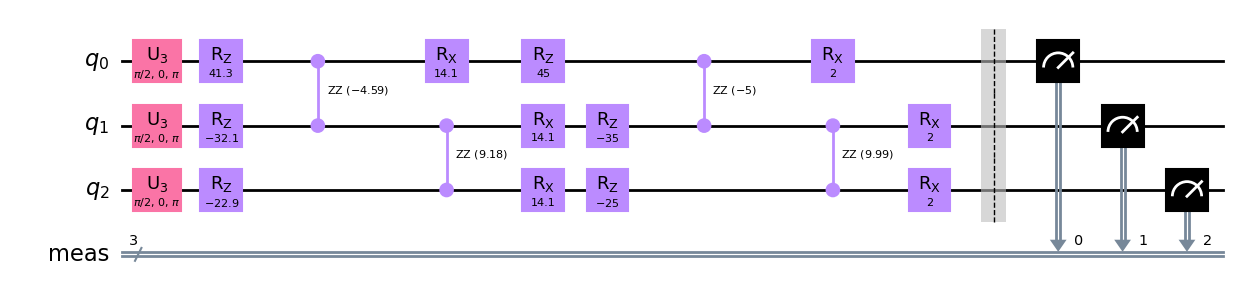
\includegraphics[width=1\linewidth]{images/qiskit_circuit.png}
    \caption{Circuit diagram with the Hadamard gates, problem Hamiltonian operator, and mixing Hamiltonian operator and  (left to right)}
    \label{qiskitcircuit}
\end{figure}
The experiments were run on the IBMQ cloud with the ibmq\_qasm\_simulator, a general-purpose simulator for simulating quantum circuits, and the COBYLA optimizer for updating the circuit parameters. We will assume an ideal circuit without a quantum noise model for measuring the optimal performance of the QAOA algorithm. We will repeatedly sample the final circuit with optimized parameters for $1000$ times and the candidate solution will be taken as the best solution among the sampled configurations.


\subsection{GUROBI Optimizer}
The GUROBI optimizer is used as a state-of-the-art classical commercial solver which is free for academic use \cite{b26}. As the GUROBI optimizer supports QUBO problems, we construct the QUBO matrix directly using the Gurobi Python library and run the optimizer locally for $10$ minutes for each input problem. If the optimizer finishes before the cutoff, the candidate solution is guaranteed to be the optimal configuration, otherwise, we would use the best solution found within the cutoff time as a candidate solution. All experiments were run with a 32 Core AMD EPYC 7543P Processor at 2.7GHz and an NVIDIA A100 40GB GPU with 500GB of RAM using Gurobi Optimizer version 10.0.3.

%All GUROBI experiments used the Gurobi Optimizer version 9.0.1 and were run on a local machine with an 8-core Apple M1 chip at 3.2GHz with 16GB of RAM.

\subsection{Fixstars Amplify QUBO Solver}
The Fixstar Amplify QUBO solver is a commercial simulated annealing-based QUBO solver that has limited free access \cite{b12}. As the Fixstar solver supports QUBO problems, we submit the QUBO matrix directly using the Fixstar API and run the solver with the highest allowed time limit which is $100$ seconds for each input problem. The solver is implemented on GPUs and is run on Fixstar remote servers which are accessed with an API token.

\section{Benchmark datasets}
We use 3 randomly generated problem sets to benchmark our QUBO solvers. These problems were chosen as they are commonly used to represent NP-hard problems to measure the performance of QUBO solvers and are relatively straightforward to encode into QUBO form. They are the not-all-equal 3-satisfiability (NAE3SAT), max-cut, and the Sherrington-Kirkpatrick (SK) model. Each problem set comprises problems of 13 sizes, ranging from $10$ to $300$\footnote{$n \in [10,15,20,25,30,35,50,75,100,150,200,250,300]$}. $20$ different random problems are generated\footnote{random seed is chosen to be from $0-19$} for each problem size $n$ for a total of $260$ problems per problem set. Each problem is also first formulated in either the QUBO or Ising form and conversion between them follows \autoref{qubotoising} and \autoref{isingtoqubo}.

\subsection*{Not-all-equal 3-satisfiability (NAE3SAT)}
The NAE3SAT problem is a variant of the boolean satisfiability problem where each problem instance consists of $n$ boolean variables $(x_1, x_2, ..., x_n)$ and $m$ clauses that each combine three literals which can be a variable or its negation. The objective is to find an assignment of boolean values such that the three values in each clause are not all the same, i.e., each clause has at least one true and one false value. The ratio of clauses to variables $\rho = \frac{m}{n}$ is a problem parameter and NAE3SAT problems are known to transition from being satisfiable to unsatisfiable at around $\rho = 2.1$ \cite{nae3sattransition}. We generate random NAE3SAT problems with $\rho = 2.1$ using the random\_nae3sat generator from the dimod Python library which "randomly samples clauses from the space of 3-variable clauses with replacement" \cite{dimodrandomnae3sat}. 

To convert a NAE3SAT problem into an Ising problem, we represent each boolean variable as a spin variable and turn each clause into a Hamiltonian term. For example, for the clause $(x_1, x_2, \neg x_3)$, we use the Hamiltonian term $H(s_1, s_2, s_3) = s_1 \cdot s_2 + s_2 \cdot (-s_3) + s_1 \cdot (-s_3)$ which has a value of $3$ when $x_1=x_2=\neg x_3$ and $-1$ otherwise. The final Hamiltonian $\Hat{H}_c$ is simply a sum of the individual Hamiltonian terms for each clause.

\subsection*{Max-cut}
The max-cut problem aims to find a partition of the vertices of a graph $G = (V, E)$ into $V_0, V_1$ with $V = V_0 \cup V_1$ and $V_0 \cap V_1 = \emptyset$, such that the number of edges crossing $V_0$ and $V_1$ is maximized. We will use the Erdos-Renyi model to generate random graphs with $n$ vertices and a probability $p=0.25$ to include each edge.

To convert a max-cut problem into a QUBO problem, we represent the assignment of each vertex as a binary variable ($x_v = i$ if $x \in V_i$) and use the objective function $f(\mathbf{x}) = \sum_{e = (u, v) \in E} -x_u - x_v + 2x_u x_v$, where each term has a value of $-1$ when $x_u  \neq x_v$ and $0$ otherwise. If a problem has a max-cut value of $C$, the objective function would have a minimum value of $-C$. 

\subsection*{Sherrington-Kirkpatrick (SK) model}
The Sherrington Kirkpatrick (SK) model is an Ising problem with a random Hamiltonian of the form $\hat{H}_c = \frac{1}{\sqrt{n}} \sum_{1 \leq i < j \leq n} J_{ij}s_i s_j$
where $J_{ij} \sim \mathcal{N}(0,1)$ are independent standard Gaussian variables. The energy landscape of the SK model is complex and has exponentially many local minima with a unique global minimum separated by high energy barriers \cite{skmodel}. This many-valley structure implies that it is extremely difficult to find the exact solution of the model. We generate random Gaussian variables with a random normal generator from the NumPy Python library.

%Parisi [6] provides a formula (for proof, see [7]) that, when numerically evaluated [8, 9, 1], shows for typical instances,
%\begin{equation*}
%    \lim_{n\rightarrow \infty} \argmin \frac{E}{n} = -0.763166...
%\end{equation*}
%(get from this paper https://quantum-journal.org/papers/q-2022-07-07-759/pdf/)

%\subsection*{Quantum Critical Points}
%get rid of Linear term
%J terms are 1
%Ising model has no linear term
%QCP is A(s)/2 = +-B(s)/2 * J magnitude is the same.
%harder for Dwave to solve, jump to excited state
%finite infinite approximating

%We plan to use a subset of the 3296 QUBO problems provided by MQLib as our benchmark dataset. These problems are publicly accessible and contain both "real-world problem instances" and randomly generated problems \cite{b12}. The dataset also contains problems of various sizes and densities. The exact benchmark dataset will be determined after further testing to determine the input limits of each solver. Each QUBO problem will first be converted into an Ising model problem and then passed to each of the solvers.

\section{Performance evaluation}
To evaluate the performance of each solver we will use two performance metrics:
\begin{enumerate}
    \item The probability of finding the best solution. The best solution is one that has the same energy as the lowest energy among all solutions found by the $5$ solvers. Since we are generating $20$ problems of each type and size, the probability for each solver is:
    \begin{equation}
        \Bar{p} = \frac{\text{number of best solutions found}}{20}
    \end{equation}
    \item The average normalized energy, used in \cite{b34}, which is:
    \begin{equation}
        \Bar{r}_{solver} =  \frac{1}{20} \sum_{i = 1}^{20} \frac{E_{max} - E_{solver}}{E_{max} - E_{min}}
    \end{equation}
    where $E_{max}$ and $E_{min}$ are the energies of the worst and best solutions found by all solvers and $E_{solver}$ is the energy that the solver found. Note that if a solver finds the best solution it gets a normalized energy of $1$ and if it finds the worst solution it gets a normalized energy of $0$. All solvers get a normalized energy of $1$ if all solutions have the same energy.
\end{enumerate}